\section{Evaluation}

\subsection{Training Datasets}
\begin{figure}
    \centering
    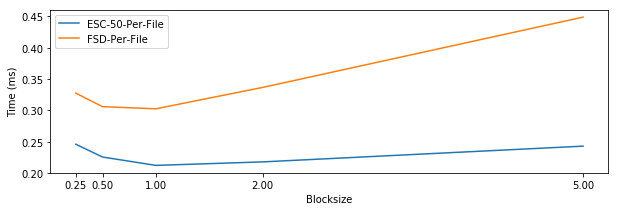
\includegraphics[width=0.45\textwidth]{figures/dataset-load-time.png}
    \caption{Caption}
    \label{fig:load-time}
\end{figure}

The datasets chosen for training are ideally clean, uniform and have about an equal number of each class instance. 

The system depends on the ability of the machine learning agent to be able to
match between acoustic features and the text queries. Its performance depends on
both the size of the database and the specificity of the query. To examine
performance across environments, we choose a clean and a dirty database: ESC-50
\cite{Piczak2015} and Freesound.
\\
\textbf{ESC-50} This clean database is made available on GitHub for environmental sound
classification. It is maintained such that the tag vocabulary is fixed and each
audio document attempts to only contains a single object in it. Each document is
5 seconds long and audio quality in terms of samplerate and recording noise is
normalized across the database. This makes for a very clean database with little
noise in both audio and annotation. It has 50 semantic classes with 40 examples
per class arranged into 5 major categories. However, the major categories do not
match the Gaver taxonomy and so were manually separated as in Table
~\cref{tab:relabel}. The database's sound documents come from the Freesound
project with the author providing uniform tags and normalizing the audio
manually \cite{Font2013}.
\\
\textbf{Freesound} The Freesound database is made up entirely of user-submitted and tagged audio documents. This is used to test the efficacy of the method on a real-world unstructured database. The documents in the database are in a variety of audio formats and lengths. Additionally, a portion of the documents contain multiple audio objects that overlap.

\subsection{Sample Balancing}
\begin{figure}[h]
    \centering
    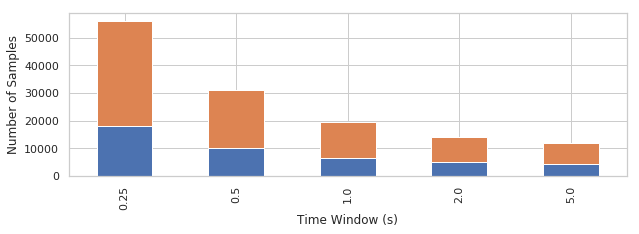
\includegraphics[width=.45\textwidth]{figures/Sample-Distribution.png}
    \caption{Sample distribution over the window sizes under consideration.}
    \label{fig:sample-distribution}
\end{figure}
Although in both the Freesound and ESC-50 database the distribution of classes is initially nearly equivalent, preprocessing alters this significantly. After extracting multiple feature vectors from the documents, the distribution much more favors some classes over other. This is likely due to the trimming of the documents of silence and differing document lengths. There are two paths to mitigate this effect: reduce the number of samples in the majority class to make them more equal or add duplicate samples from the minority class. Both of these approaches have risks associated with them, namely a loss in generalizability, \cref{fig:sample-distribution} illustrates the exponential relationship between window size and distribution of unbalance for the topmost classes of the hierarchy.

To determine the optimal approach for supersampling or subsampling, we train RFCs as they are the most of the classifiers used to overfit with duplicates. The classifiers trained on these sets are compared to the AUC-ROC curve of an unbalanced training set to identify the most optimal approach.

\subsection{Window Size}

Choosing the size of the window determines the granularity of the feature vector as each window's feature matrix is reduced into a vector for training. If the window is too large we obtain a single feature vector, but it is likely too generic to be useful in classification. On the other hand, a window that is too small will increase the time required to complete preprocessing, training, and evaluation steps and increase the size of the feature table. To determine the optimal window size, we evaluated five window sizes with each high-level classifier. The optimal window size is the one that balances training time, evaluation time, classification accuracy, and classifier confidence.

\begin{figure}[h]
    \centering
    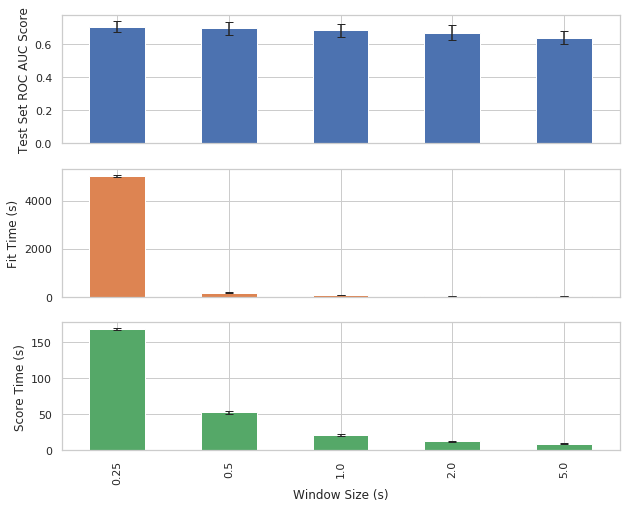
\includegraphics[width=.48\textwidth]{figures/ROC-AUC-Window-Compare.png}
    \caption{Comparison of window sizes across three metrics.}
    \label{fig:roc-auc-window}
\end{figure}

The first experiment trained an SVM classifier with default hyper-parameters on the highest level of the hierarchy for each time window size to determine which window is the most clearly separable. The classifier was then tested with 10-fold cross-validation on the entire dataset and the mean and standard deviation of the fit time, score time, and ROC AUC score over all 10 folds were collected. As seen in \cref{fig:roc-auc-window}, the classifier performs best on a quarter-second window however the amount of time necessary to both score and fit a classifier to the dataset much larger than that of even a half-second window. here, we see that the second best choice of a half-second window performs about as well and does not have as large of a fitting and scoring cost. Though, one may be tempted to use the five second window as it has the lowest fit and scoring time across all windows, however our classification confidence tests show this approach to be sub-optimal.

\subsection{Hierarchical Classifier}

\subsubsection{Comparison with Baseline}
Here, we compare the performance of standard classification techniques with the hierarchical approach.

\subsubsection{Convolutional Neural Network}
Here, we compare performance of CNNs with that of the hierarchical approach.


\subsection{Dimensionality Reduction}
The standard length of the feature vector derived from each audio file is 129 values, causing training time to suffer from the curse of dimensionality. To mitigate this effect a combination of feature selection and reduction techniques are used. The initial feature columns are reduced by selecting the top K features, measured by some heuristic (e.g. chi, information gain, gini). The remaining features are then transformed by a feature reduction technique (e.g. ICA, PCA, LDA) to find a better projection of the data for classification.

\subsection{Filtering Classifier}
As stated before, the filtering classifier has much different goals than that of the deciding classifier and as such has a different heuristic of optimality. The optimal classifiers in this case value scoring time and uncertainty in misclassification over pure accuracy performance.

\subsubsection{Training}
Each of the subcategories in the hierarchy were individually trained, determining their optimal classifier. This means an extra training cost is incurred for each interim classifier. We also consider the propagation of error in hierarchical classifiers when choosing an optimal classifier. As shown in our window size tests, some probabilistic representations are more or less confident in classification. We aim to have as little confidence as possible in misclassified results for these classifiers. This is done even to the detriment of confidence in correct classifications.

\subsubsection{Evaluation}

\subsection{Deciding Classifier Training}
The deciding classifier's goals are more in line with those of traditional classifiers. The training and evaluation time of this classifier is much less important than its classification accuracy and precision. This is due to the idea that the evaluation task will be executed on much fewer documents than the filtering classifiers.

\subsubsection{Training}

\subsubsection{Evaluation}

\begin{figure}[h]
    \centering
    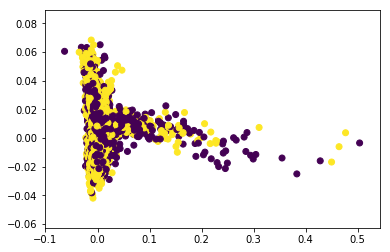
\includegraphics[width=0.45\textwidth]{figures/pca-cluster-hl.png}
    \caption{2D clustering of features using PCA.}
    \label{fig:pcahl}
\end{figure}


\begin{figure}
    \centering
    \includegraphics[width=0.45\textwidth]{example-image-a}
    \caption{Comparative training time between PAMIR, WARP, and ECHO (what we're calling this system?)}
    \label{fig:my-label}
\end{figure}

\begin{figure}
    \centering
    \includegraphics[width=0.45\textwidth]{example-image-a}
    \caption{Plot of training iterations needed before getting diminishing returns (comparative between classifiers)}
    \label{fig:learning-curve}
\end{figure}

\subsubsection{Representation Experiments}

\begin{table}[]
    \begin{tabular}{llllll}
    Classifier/Window       & 250 ms & 500 ms & 1 s   & 2 s  & 5 s   \\
    Deep Neural Nets        & 0.628  & 0.653  & 0.656 &      &       \\
    Random Forest           & 0.66   & 0.68   & 0.68  & 0.64 & 0.69  \\
    K-Nearest Neighbors     & 0.61   & 0.62   & 0.62  & 0.65 & 0.64 \\
    Support Vector Machine  & 0.62   & 0.64   & 0.62  & 0.62 & 0.67   
    \end{tabular}
\end{table}

Classifier performance at different window sizes and features (remember, have run wavenet)

\begin{figure}[h]
    \centering
    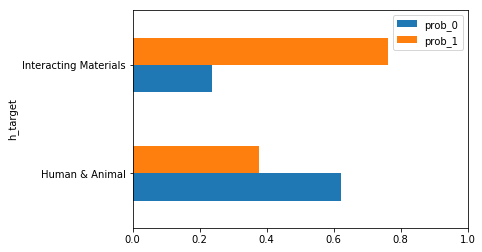
\includegraphics[width=0.45\textwidth]{figures/knn-prob-plot.png}
    \caption{Plot of average probabilities for each class of the misclassified documents at the top level.}
    \label{fig:a}
\end{figure}

\subsubsection{High-Level Classification}

\begin{figure}
    \centering
    \subfloat[SVM]{{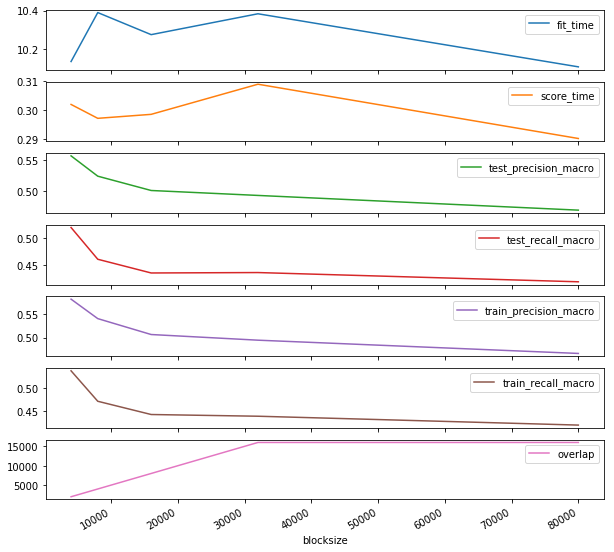
\includegraphics[width=0.25\textwidth]{figures/FSD-SVM.png}\label{fig:fsd-svm}}}
    \subfloat[KNN]{{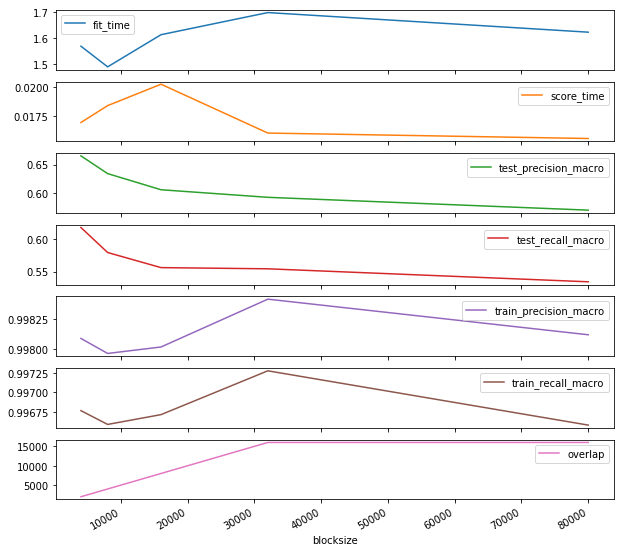
\includegraphics[width=0.25\textwidth]{figures/FSD-KNN.png}\label{fig:fsd-knn}}}
    \hfill
    \subfloat[RFC]{{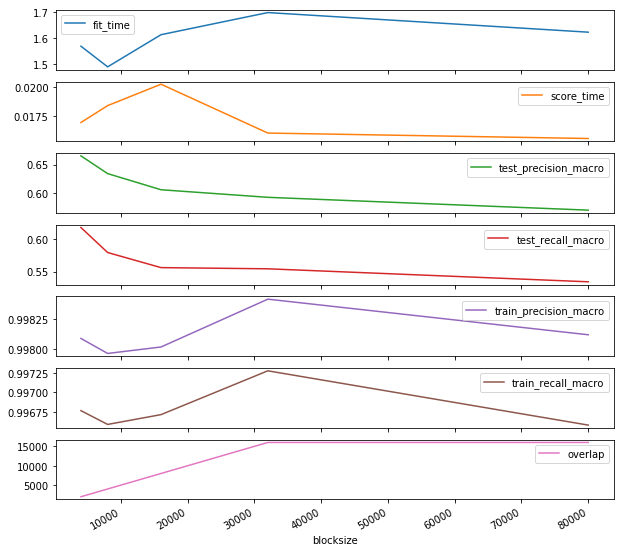
\includegraphics[width=0.25\textwidth]{figures/FSD-RFC.png}\label{fig:fsd-rfc}}}
    \caption{Training and testing statistics of high level classifiers on the FreeSound Database.}
\end{figure}

\begin{figure}
    \centering
    \subfloat[SVM]{{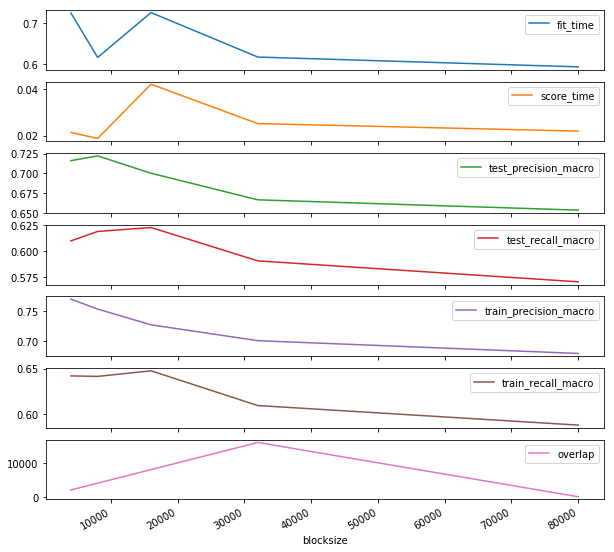
\includegraphics[width=0.25\textwidth]{figures/ESC-50-SVM.png}\label{fig:esc-50-svm}}}
    \subfloat[KNN]{{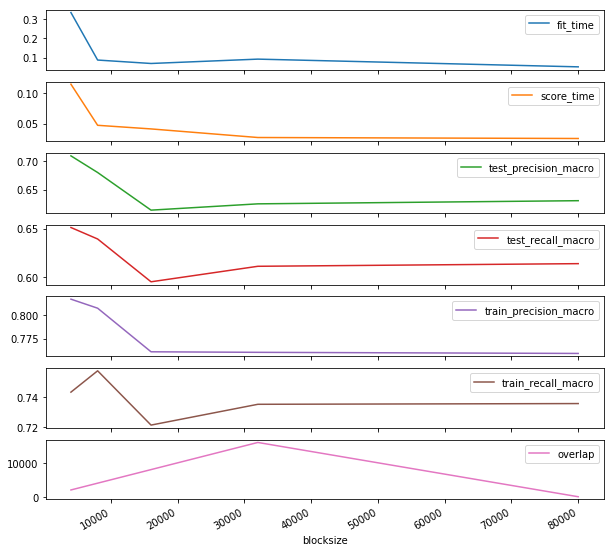
\includegraphics[width=0.25\textwidth]{figures/ESC-50-KNN.png}\label{fig:esc-50-knn}}}
    \hfill
    \subfloat[RFC]{{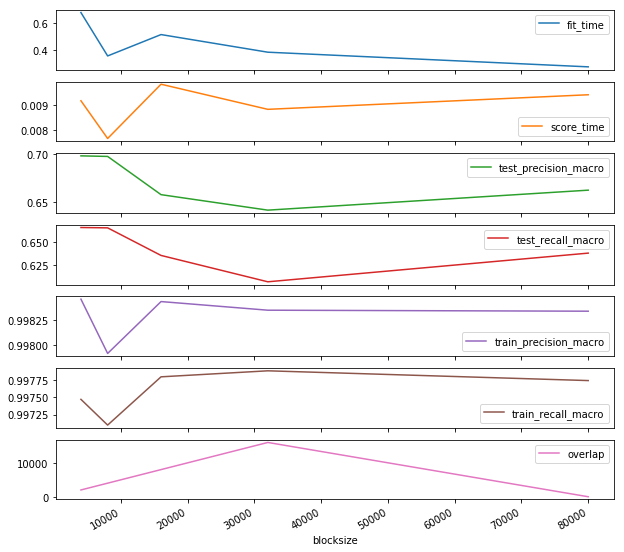
\includegraphics[width=0.25\textwidth]{figures/ESC-50-RFC.png}\label{fig:esc-50-rfc}}}
    \caption{Training and testing statistics of high level classifiers on the ESC-50 Database.}
\end{figure}

\subsubsection{Low-level Classification}

\begin{figure}
    \centering
    \subfloat[SVM]{{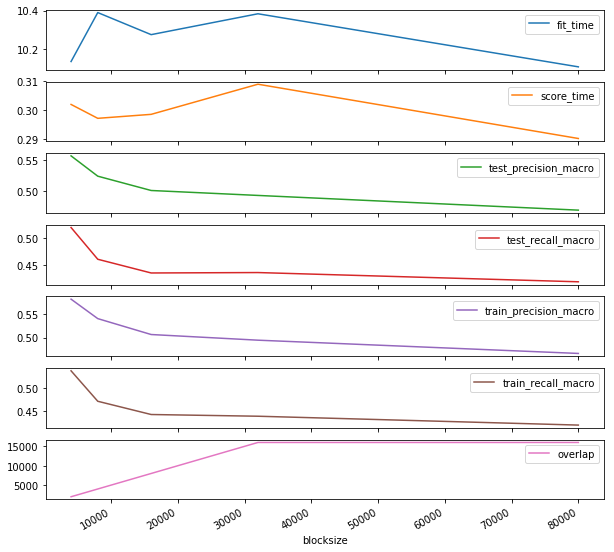
\includegraphics[width=0.25\textwidth]{figures/FSD-SVM.png}\label{fig:fsd-svm}}}
    \subfloat[KNN]{{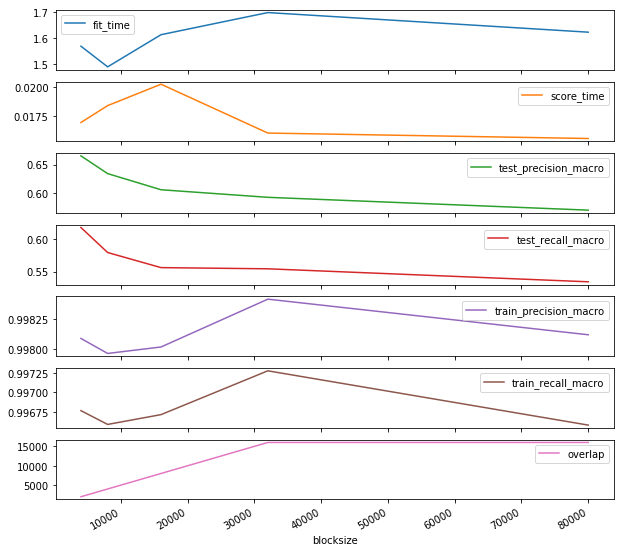
\includegraphics[width=0.25\textwidth]{figures/FSD-KNN.png}\label{fig:fsd-knn}}}
    \hfill
    \subfloat[RFC]{{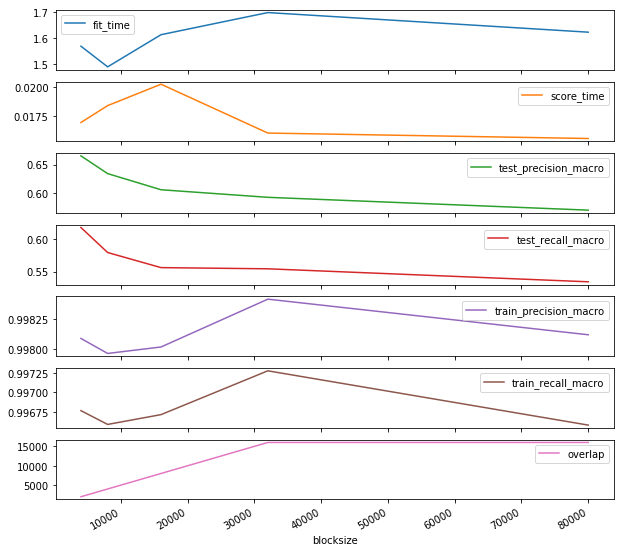
\includegraphics[width=0.25\textwidth]{figures/FSD-RFC.png}\label{fig:fsd-rfc}}}
    \caption{Training and testing statistics of high level classifiers on the FreeSound Database.}
\end{figure}

\begin{figure}
    \centering
    \subfloat[SVM]{{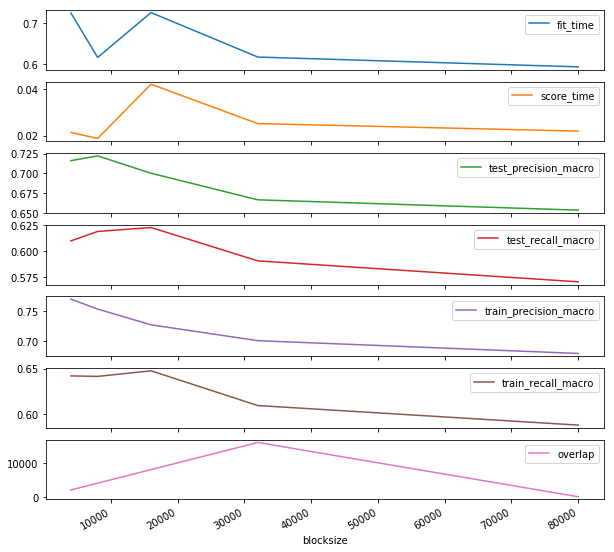
\includegraphics[width=0.25\textwidth]{figures/ESC-50-SVM.png}\label{fig:esc-50-svm}}}
    \subfloat[KNN]{{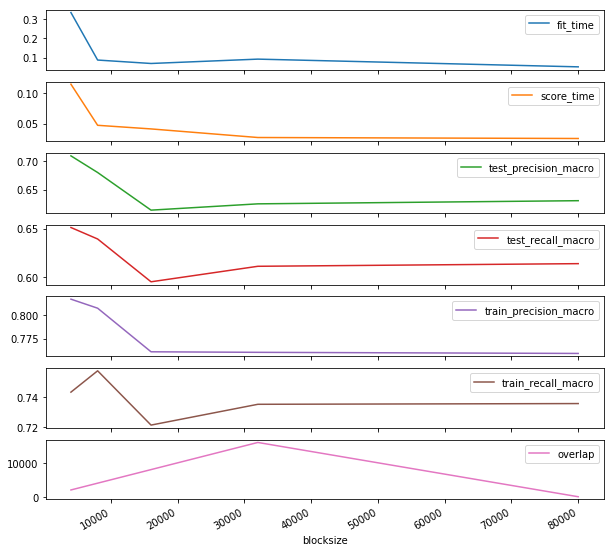
\includegraphics[width=0.25\textwidth]{figures/ESC-50-KNN.png}\label{fig:esc-50-knn}}}
    \hfill
    \subfloat[RFC]{{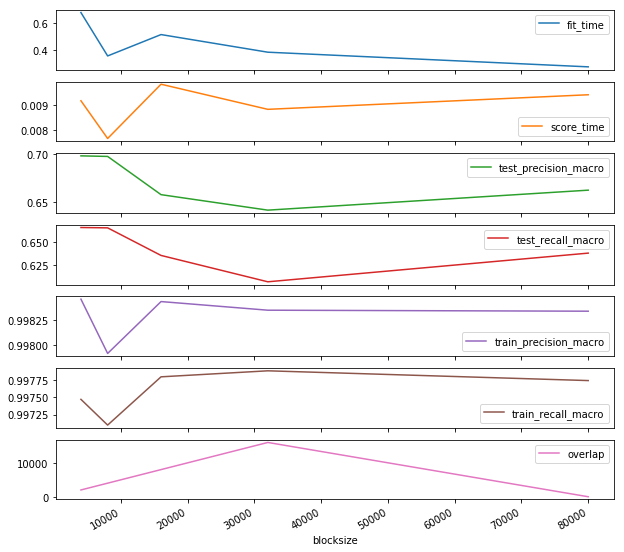
\includegraphics[width=0.25\textwidth]{figures/ESC-50-RFC.png}\label{fig:esc-50-rfc}}}
    \caption{Training and testing statistics of high level classifiers on the ESC-50 Database.}
\end{figure}

\subsubsection{Full Classification Performance}

Cross-validated performance of each subclassifier and performance of hierarchical

\subsubsection{Retrieval Performance (Time + Accuracy)}


\section{Conclusion}
The approach here shows promise, especially in the context of a retrieval
system. Using human perception as a model is an approach that had been pursued
in machine vision with success and it is only logical to do the same for machine
listening. By understanding the mechanisms by which we convert auditory signals
to brain signals, we can understand how the audio needs to be encoded for use in
machine hearing. One of the aspects of audio we have yet to optimally integrate
are temporal features which are of utmost importance in audio signals.

To this end, several representations were attempted in this work. The first was
just basic feature extraction from spectral representations of the audio using
librosa. Librosa allowed for many spectral and temporal features to be taken
from the signal though it is a slow process and may still not provide a good
feature set. To better emulate human perception, auto-encoders were attempted
next. The thought was that a neural network will be able to find latent
variables that are of better use than those extracted from usual means. However,
it was found that this approach did not bear out and hardly effected
performance.

Experiments were run comparing this approach to two off-the-shelf classifiers on
each layer of the hierarchy. The SVM classifier consistently under-performed and
will likely be removed from subsequent evaluations. A Random Forest Classifier
was consistently about equal to the neural networks it was evaluated against but
in nearly every case, the network was able to beat its precision score.

Overall, this study provided insights into the complexity of autonomous audio
analysis and the challenges that are still facing the field. of these
challenges, it seems that representation is the most pressing. It appears though
that the current direction of studying human perception mechanisms and emulating
them will prove optimal.

